\section{Experimental Studies}

To provide a first experimental evaluation of BTM, we asked two questions:
\begin{itemize}

\item Does BTM identify errors efficiently?

\item Can we use the discovered errors to improve the models?

\end{itemize}

For our experiments, we used the BTM system to challenge two
classification systems. One for detecting pages with hate speech, and
one for detecting pages with adult content. We ran the systems with
the configuration details described in the previous section (1 cent
for the base task, 50 cents maximum payment for a URL that generates
an error).

\textbf{Comparison with stratified random testing:} For the two systems, we compared BTM with the usual quality assurance process of examining the output of the classifier to identify errors.  Examining a uniform random sample of the output is particularly uninformative, as the classifiers are quite accurate and the distributions are quite unbalanced, and so the vast majority of cases are correctly classified and not objectionable.  Therefore, standard procedure is to examine a random sample, stratified by the model's confidence score.  Specifically, the range of confidence scores [0,1] was divided into $k$ equal-width bins.  A set of $N$ URLs for testing was sampled randomly, with $\frac{N}{k}$ from each bin.  This stratification is used because it generally finds more errors, because it over-samples the URLs for which the models have low confidence (and are likely to be wrong).  However, the discovered errors are likely to be ``known unknowns.''  

For the adult classifier, the human workers identified errors in 16\%
of the inspected cases (\textit{much} higher than the natural error
rate of the classifier).  In contrast, using BTM, more than 25\% of
the submitted cases generated an error (a 56\% increase). The
corresponding statistics for hate speech favored BTM even more
strongly: workers identified errors only in 9\% of the inspections for
stratified random sampling, but they identified errors in 27\% of the
URLs with BTM (three times as many). 
\foster{Insert a projection of the rate of finding UUs for (1) random sampling, and (2) if the stratification were all on the top bucket.  Add these estimations to the bar charts.}
These results indicate that the BTM process is indeed
more efficient than the standard evaluation procedure in identifying
problematic cases.  It should be noted that we could increase the
``efficiency'' of the non-BTM procedure by simply sampling more from
the low-confidence cases.  However, this would directly reduce the
number of ``unknown unknowns'' discovered.  At the extreme, the
largest number of errors would be found by sampling only in the
low-confidence region.  All the errors found would then be known
unknowns.  So, let's now consider the effect of BTM on the severity of
the errors found.

\textbf{Comparing the severity of errors:} Figure~\ref{fig:hate-speech} and~\ref{fig:adult} show the distribution of modeling mistakes identified for hate speech and adult content tasks, respectively. A consistent behavior is observed for both categories: BTM identifies a significantly larger number of severe misses---the unknown unknowns. Within the errors identified by BTM, 25\% were cases of high severity; the model was confident that it was making the correct decision (classifying the content as benign, with 100\% confidence), but in reality the decision was incorrect. So, not only does BTM identify a larger number problematic cases than the stratified testing, but also a significant number of these cases were unknown unknowns: cases that would be missed and without a very unpleasant event (possibly a catastrophe), we never would know that we missed them. In contrast, and by now as expected, most of the identified 
errors for the stratified random sampling were near misses that occur near the decision boundary.

\begin{figure}[t]
\centering
\center{
\subfigure[Hate Speech]{
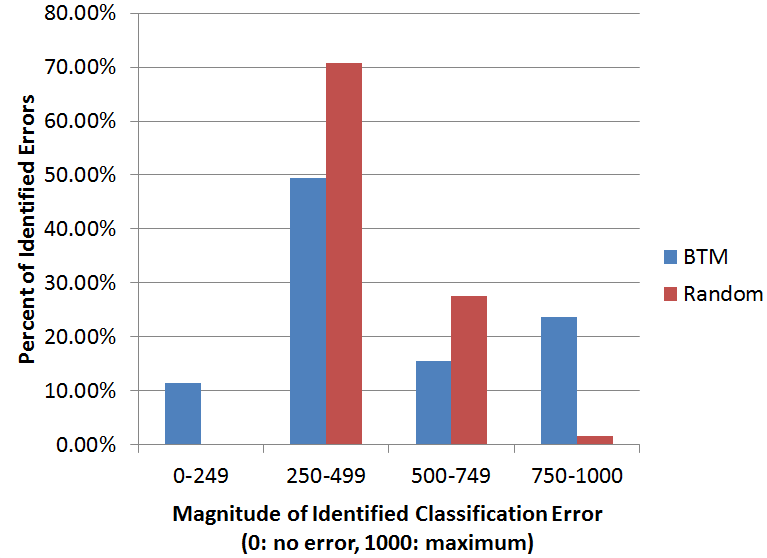
\includegraphics[width= \columnwidth]{plots/Hate-speech-scores.PNG}
\label{fig:hate-speech}
}
\subfigure[Adult Content]{
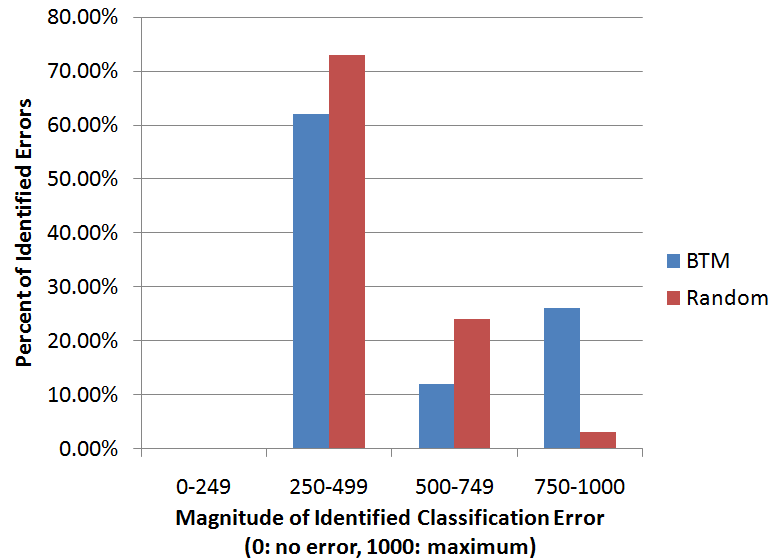
\includegraphics[width= \columnwidth]{plots/porn-scores.PNG}
\label{fig:adult}
}
\caption{Distributions of the magnitude of the identified mistakes in the predictive model's output by BTM and by random sampling for two ad safety tasks.  Each bar indicates the percentage of successfully identified mistakes that reside in the associated score range.}
}
\label{fig:results}
\end{figure}

\drop{
\begin{figure}[t]
\center{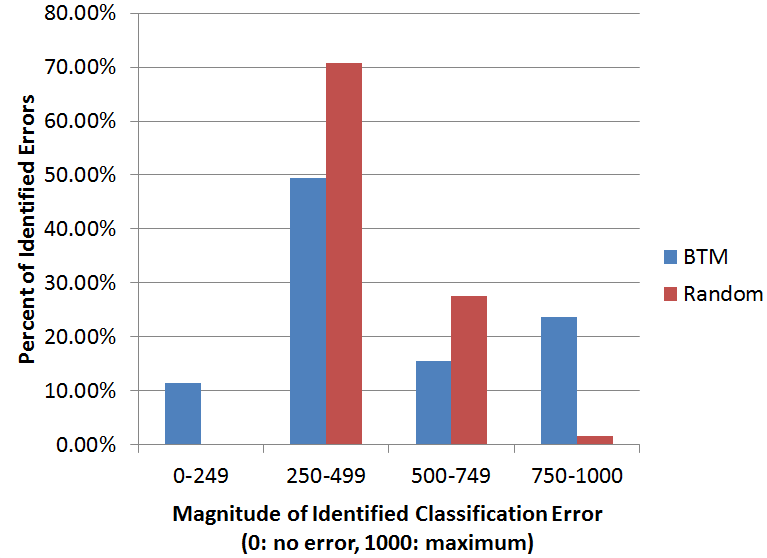
\includegraphics[width=\columnwidth]{plots/Hate-speech-scores.PNG}}
\caption{A distribution of the magnitude of the identified errors by BTM and by random sampling for the hate speech category.}
\label{fig:hate-speech}
\end{figure}

\begin{figure}[t]
\center{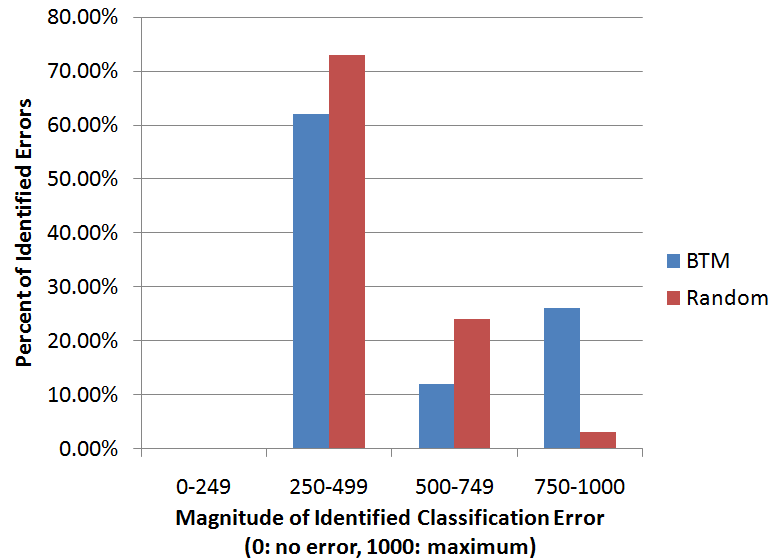
\includegraphics[width=\columnwidth]{plots/porn-scores.PNG}}
\caption{A distribution of the magnitude of the identified errors by BTM and by random sampling for the adult content category.}
\label{fig:adult}
\end{figure}
}

\textbf{Learning from identified errors:}  A natural question to ask is if the cases found by BTM seem to be isolated outliers, or whether they seem to be regularities that can be modeled. To this end we ran the following experiment: We attempted to learn a model that would classify positive and negative examples from amongst the BTM-identified cases.\footnote{That is, false negatives and false positives from model being considered, respectively } Internal consistency in the identified errors would suggest that these cases are not outliers, but rather constitute parts of the space where the model fails systematically (potentially without being aware of the failures).


Figure~\ref{fig:curves} shows the results of this process. The ``btm
only'' line shows the quality of the model built and tested using the
error cases identified by the BTM process.  The ``student only'' line
shows the quality of the model built and tested using examples
gathered through stratified random sampling (the pages selected
through random sampling were inspected by students, hence the
name). Both the btm-only and student-only lines show quality
measurements computed via cross-validation.  
Importantly, the results show that the
quality of both models is fairly high.  This illustrates that there is
consistency and internal coherence in these sets pages.  The fact that
the BTM model can reach high levels of accuracy indicates that BTM
indeed identifies systematic errors, and not just disparate outliers.
However, note the difference between the quality that is achievable by training with the two different data sets.  
The comparatively lower quality of the random sampling model
illustrates that these pages are inherently more difficult to learn
from; this is consistent with our discussion above that the discovery
via stratified random sampling (DVSRS) focuses on the ambiguous cases
(those that the current model is uncertain about), while BTM discovers
incorrectly classified areas of the space that have been
systematically ignored.

We also can examine whether the two approaches (DVSRS and BTM) identify sets of similar examples, or whether each of them identifies something completely different. For that, we tested the performance of BTM using the examples from DVSRS (``student'') and vice versa. The results indicate that there is little cross-consistency between the models. What we discover using BTM has little effectiveness for classifying the error cases identified through DVSRS, and vice versa. This finding indicates  that BTM reveals errors in parts of the space unexplored by DVSRS.

BTM and DVSRS seem to be different processes, capable of identifying different types of errors. Each of these has its place in the evaluation and improvement of automatic models. DVSRS identifies primarily cases where the model already knows that it is not confident. 
The results show that even if the DVSRS were stratified only on the ``unknown'' region, it still would not identify nearly as many unknown unknowns as Beat the Machine.
The BTM process, through its game-like structure and probing nature, encourages the discovery of unknown problems in the model. The fact that humans can easily find challenging cases for the automatic models, when being themselves confronted with this challenge, also indicates that human expertise and curiosity can improve even very accurate automatic models.



\begin{figure}[t]
\center{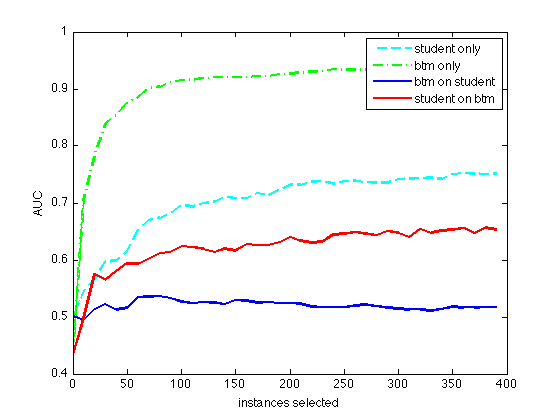
\includegraphics[width=\columnwidth]{plots/adt_btm_eval.png}}
\caption{Learning curves generated by the models
using cross-validation (BTM and student lines), and then use as test case for BTM the errors identified by random sampling (BTM on students), and vice versa (students on BTM).}
\label{fig:curves}
\end{figure}


